\documentclass[11pt, a4paper, oneside]{ctexart}
\usepackage{amsmath, amsthm, amssymb, appendix, bm, graphicx, hyperref, mathrsfs}
\usepackage{fancyhdr}%导入fancyhdr包
\usepackage{ctex}%导入ctex包
\usepackage{geometry}
\usepackage{setspace}
\usepackage{graphicx}
\usepackage{pythonhighlight}
\usepackage{scalerel}
\usepackage{listings}
\usepackage{ctex}
\usepackage{graphicx}
\usepackage{setspace}
%\usepackage[a4paper, body={18cm,22cm}]{geometry}

\usepackage{float,abstract,booktabs,indentfirst,amsmath}
\usepackage{array}
\usepackage{booktabs} %调整表格线与上下内容的间隔
\usepackage{multirow}
\usepackage{url}
\usepackage{diagbox}
\renewcommand\arraystretch{1.4}
\usepackage{indentfirst}
\setlength{\parindent}{2em}

\usepackage{listings}
\usepackage{xcolor}

\renewcommand{\baselinestretch}{1.5}
%\geometry{left=2.8cm,right=2.8cm,top=2.5cm,bottom=2.5cm}
%\geometry{left=3.18cm,right=3.18cm,top=2.54cm,bottom=2.54cm}
\geometry{left=3.10cm,right=3.18cm,top=3.14cm,bottom=2.5cm}

\pagenumbering{arabic}%设置页码格式,大写字母标页
\pagestyle{fancy}
\fancyhead{} % 初始化页眉
\fancyhead[R]{\small{王治平\ 320200908151}}
\fancyhead[L]{\small{双原子分子振动能级半量子化理论的数值计算}}
\fancyfoot{} % 初始化页脚
%\fancyfoot[LO]{奇数页左页脚}
%\fancyfoot[LE]{偶数页左页脚}
%\fancyfoot[RO]{奇数页右页脚}
%\fancyfoot[RE]{偶数页右页脚}
\fancyfoot[R]{\thepage}
\renewcommand{\headrulewidth}{0.8pt}%分隔线宽度4磅
\renewcommand{\footrulewidth}{0pt}
\title{\textbf{双原子分子振动能级半量子化理论的数值计算}}
\begin{spacing}{0}

\author{{王治平} 
\\\vspace{-6mm}
\small{2020级\ \ 物理学二班}
\\\small{320200908151}
\\{指导老师:吴枝喜、关剑月}}
    %%行间距变为double-space
\end{spacing} 
\date{\today}
\linespread{1.5}
\newtheorem{theorem}{定理}[section]
\newtheorem{definition}[theorem]{定义}
\newtheorem{lemma}[theorem]{引理}
\newtheorem{corollary}[theorem]{推论}
\newtheorem{example}[theorem]{例}
\newtheorem{proposition}[theorem]{命题}
\renewcommand{\abstractname}{\Large\textbf{摘要}}




\begin{document}
\maketitle
	%\tableofcontents
	
	%\begin{center}
		%\LARGE{{\textbf{\heiti 实验一 远程过程调用中间件及数据访问中间件}}}
		%\newline
		%\newline
		%\date{2019年4月2日}
		%\begin{table}[H]
		%	\centering
		%	\begin{tabular}{p{3cm}p{4cm}<{\centering}p{3cm}p{4cm}<{\centering}}
		%		班\quad 级: & 2020级物理学一班 & 学\qquad 号:   & 320200908151 \\ \cline{2-2} \cline{4-4}
		%		姓\quad 名: & 王治平       & 指导老师: &吴枝喜、关剑月       \\ \cline{2-2} \cline{4-4} 
		%	\end{tabular}
		%\end{table}
	%\end{center}

    \maketitle

    \setcounter{page}{0}
    \maketitle
    \thispagestyle{empty}
    ~\\~\\~\\

\maketitle

\setcounter{page}{0}
\maketitle
\thispagestyle{empty}

\begin{abstract}
    {
        量子系统的能级问题通常都
        是通过对于$Schrödinger$方程来求解进行处理。
        这种常规方法,可以同时给
        出系统的束缚态能级和相应的本征函数,
        然而对于一些系统能直接求解较为困难,常
        采用数值法或各种不同的近似方法 .
        本文采用了以$Lennard-Jones$势和
        $Morse$势两种位势函数近似描述双原
        子分子振动过程的势能,从而求解。
        文章给出了两种位势函数作为理论支持下
        数值计算的初步结果,对其分别分析了的误差
        结果差异与初步原因,并指出了两种函数各自
        的问题。


    }
\end{abstract}

\vspace{45mm}\begin{center}
    \small{课题程序实现已上传至}\footnotesize{https://github.com/YingD0/level2-work1}
        
\end{center}

\newpage
\pagenumbering{Roman}
\setcounter{page}{1}
\tableofcontents
\newpage
\setcounter{page}{1}
\pagenumbering{arabic}

\section{课题介绍}
\subsection{分子振动能级}
{分子能级指的是分子内部各种运动状态所形成的能级结构,
分子内部各种运动状态所形成的能级结构,其内部的运动有
电子运动、分子振动和分子转动,它们的能量都是量子化的,
故可形成电子能级、振动能级和转动能级。其中振动能级能
级跃迁产生振动光谱,有一定的宏观表现。%分子的电子能级为10电子伏特(eV)量级,与原子的能级差不多;分子的振动能级大约是电子能级的0.1倍,分子的转动能级大约是电子能级的m/M倍,其中m是电子的质量,M是典型分子的质量。由于典型分子的质量比电子质量要大数千倍至万倍,从而分子振动能级为0.电子伏特(eV),转动能级为0.001eV,因此分子的能级比原子的能级复杂,由此决定分子比原子具有丰富得多的光谱。}
\subsection{课题内容}
{本课题旨在对模式分子\footnote{本文中模式分子指具有典
型性质便于数值计算的简单上双原子分子,如$H_2$,  $ DH $,  $O_2$等}的振动能级进行数值
计算,期间用到\emph{Bohr}等人的半量子理论进行分析架构,故为双
原子分子振动能级半量子化理论的数值计算。}
\newpage
\section{理论分析}
\subsection{原理介绍}
\subsubsection{\emph{Bohr}的定态能级假设}
{1913年,为了解释氢原子的线状光谱,\emph{Bohr}作出以下三个假设:
}


\setlength{\parindent}{3em}
{
$\bullet${\bfseries{定态假设:}}{电子仅沿特殊轨道圆周运动, 此时其处于不辐射电磁波的
具有确定能量$E_n$的稳定状态, 称作定态。}


$\bullet${\bfseries{跃迁假设:}}{当电子在两个定态
$E_m$和$E_n$跃迁时, 才伴有频率为 $\nu=|E n −
E m |/h$的电磁波的吸收或发射。}


$\bullet${\bfseries{量子化假设:}}{
运动轨道由量子化条件$J =\oint pdq = 
nh $(n 为非负整数) 确定, 其中
J 为电子角动量, p 和 q 分别为其广义动量和广义
坐标}
}

\setlength{\parindent}{2em}{本次课题主要利用\emph{Bohr}的定态能级假设
中的量子化假设作为理论基础,结合基础物理学定律
进行数值计算。结合本体具体情况量子化假设可以表示为在
相空间中闭合轨道积分满足闭合积分(相空间面积)为$\hbar/2$
的奇数倍,即$\oint pdr = n+\frac{1}{2} \hbar $
具体理论会在2.1.3部分讨论。}
\subsubsection{原子核势能}{
    考虑一维空间中孤立双原子分子的运动,由于原子核对于
    核运动的贡献远大于核外电子,故而在本题目的讨论中可
    以仅讨论原子核的能量。由于其运动过程中所受的作用力
    的大小以及种类与其核间距(r)有关(近距离主要为电磁作用
    和
    量子作用,远距离主要为范德瓦耳斯作用以及电磁作用)
    ,故而可以用一个关于核间距的函数表示这种相互之间的
    位势。通常用来表示上述关系的势函数有\emph{Lennard-Jones}
    位势,\emph{Morse}位势,以及\emph {Varshni}
    经验势,其中本文采用前两种势函数进行数值计算与结果比较。


$\bullet${}\bfseries{\emph{Lennard-Jones}势}}


{
    最早由数学家{\emph John Lennard-Jones}于1924年提出。由于其
    解析形式简单形象而被广泛使用,其表达式为
\begin{equation}
    V(r)=V_0[(\frac{a}{r})^{12}-(\frac{a}{r})^6]
\end{equation}


{其中r为两原子核之间的距离,$V_0$为势井深度,a为波尔
    半径。绘制出的无量纲示意图见\ \emph{图1}.}
}

{
    \begin{center}
          
        \begin{figure}[ht]\vspace{-2mm}
            \begin{minipage}[t]{0.5\linewidth}
            \centering
            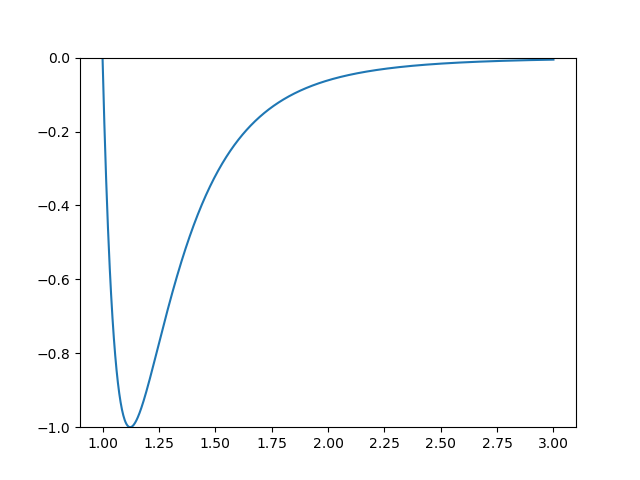
\includegraphics[scale=0.5]{1.png}\vspace{-6mm}
            \caption{\small{ $Lennard-Jones$势-核间距无量纲化图像}}
            \end{minipage}%
            \begin{minipage}[t]{0.5\linewidth}
            \centering
            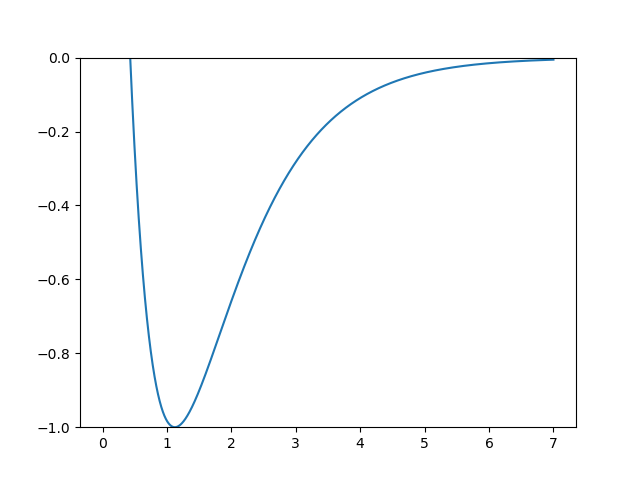
\includegraphics[scale=0.5]{2.png}\vspace{-6mm}
            \caption{\small{ $Morse$势-核间距无量纲化图像}}
            \end{minipage}
        \end{figure}
    \end{center}    
}
\vspace{-8mm}
$\bullet${\bfseries{\emph{Morse}势}}


{
    以物理学家\emph{Hilip M. Morse}的名字命名的Morse势是
    一种对于双原子分子间势能的简易解析模型。 一方面,对
    \emph{Morse}势求解薛定谔方程具有解析解,方便分析问题;另
    一方面,由于它隐含地包括了键断裂这种现象,对于分子
    振动的微细结构的具有良好的近似。Morse势包含有谐振
    子模型所缺乏的特性,那就是非成键态。相对量子谐振子
    模型,\emph{Morse}势更加真实,因为它能够描述非谐效应,倍
    频,以及组合频率。

    \emph{Morse}势具有如下的形式
\begin{equation}
    {V(r)=-D_{e}+D_{e}(1-e^{-a(r-r_{e})})^{2}}
\end{equation}


{在这里,$r$是核间距(或键长
);$r_e$是平衡键长(
{$\frac{dV(r)}{dr}|_{r=r_{e}}=0$},即最低
点对应r值);
{$D_{e}$}是Morse势的阱深(势能零点可任意选
取,在此将解离极限设为势能零点,即两核间距
趋于无穷远时令
系势能为零),{$V(\infty )=0$});
{$a$}则控制了势井的“宽度”,然而在本题中只考虑纵向能级
,故可暂且不与讨论。对于$Morse$势绘制出的无量纲示意图
见\ \emph{图2}.
}


\subsection{理论生成}
{基于上述两个前置介绍,我们可以得到分子振动的势能以及总
能量,仅仅讨论振动能级时我们可以对于能级计算进行简化,
并得出简化模型的计算方法。}
\subsubsection{简化模型}
{
$\bullet${\bfseries{只考虑原子核的运动}}

{\setlength{\parindent}{3em}同2.1.1介绍,在本题目尺度要求下,可以省却电子运动的影响
故而将势能简化为原子核势能,便于后续的分析与讨论。}

$\bullet${\bfseries{只考虑原子核的振动}}

{\setlength{\parindent}{3em}原子核占有原子绝大多数
的质量,同时原子核的转动比振动要慢的多,故而对于振动能级
的贡献可以忽略,故而可以作出只考
虑原子核的振动。}

$\bullet${\bfseries{振动方程的讨论}}

{\setlength{\parindent}{3em}原子核尺度的粒子运动可以用
量子力学理论进行解释,设第$n$能级的振动能量为$E_n$,
波函数为$\Psi_n(r,t)$,简化后的核的振动可以用一维定态薛
定谔方程描述
\begin{equation}
	[-\frac{\hbar^2}{2m}\frac{d^2}{dr^2}+V(r)]\Psi_n=E_n\Psi_n
\end{equation}
\par 按照量子理论只需要解出$[-\frac{\hbar^2}{2m}\frac{d^2}{dr^2}+V(r)]$在波函数空间中的本征值,
这样就得出了各能级以及对应能量。本题我们把问题看作原子核在\emph{V(r)}势场的经典运动
结合\emph{Bohr}的定态能级假设来求解量子化的振动能级。
}

\subsubsection{理论生成}
{
    有了上述的简化模型,我们可以进行一些简单的理论分析。

    从能量角度,系统具有的总能量为
\begin{equation}
E=\frac {p^2}{2m}-V(r)
\end{equation}


    \emph{p}为原子核相对运动的动量,
    $m=\frac{m_0^2}{m_0+m_0}=\frac{1}{2}m_0$
    为约化质量。显然前一项为动能项,后一项为势能项。

    根据(4)式\emph{p}可以写作如下形式。
    \begin{equation}
        p(r)=\pm\sqrt{[2m(E-V(r))]}
    \end{equation}

    显然的,在确定能级下(给定$E$)这是一条在相空间的闭合
    轨道。由{\emph{Bohr}的定态能级假设}的限
    制我们可以得到
    \begin{equation}
        \oint p(r)dr=({2n+1)}\pi \hbar
    \end{equation}
    
    将(5)式代入,同时用$E_n$表示第$n$级轨道对应的能量
    ,考虑到p的方向性每个确定态具有两个相反的取值,得到如
    下方程
    \begin{equation}
        \int^{r_{out}}_{r_{in}}\sqrt{2m(E_n-V(r))}dr=(n+\frac{1}{2})\pi\hbar
    \end{equation}

    其中$r_{in}$,$r_{out}$表示相空间左右两
    个端点,根据相空间物理意义可知其为运动的两
    个极限点,此刻动能全部转化为势能,即
    $E_n-V(r)=0$。

    为了减少计算工作量,防止数据溢出,同时也
    我们对上述提到的物理量进行无量纲化:

    \begin{center}
        {$\varepsilon_n =\frac{E_n}{V_0},\ \ x=\frac a c ,\ \ \gamma=\sqrt{\frac{2ma^2V_0}{\hbar^2}}$}
    \end{center}

    
    (7)式可以改写为
    \begin{equation}
        \gamma \int ^{x_{out}} _{x_{in}}\sqrt{\varepsilon_n-v(x)}\ dx=(n+\frac 1 2 )\pi
    \end{equation}

    其中
    \begin{center}
        $v(x)=4(x^{-12}-x^{-6})\quad (Lennard −Jones $势)\end{center}
        
        
        或

\begin{center}
        $v(x)=-1+(1-e^{-a(x-x_{e})})^2\qquad (Morse$势)
    \end{center}

    在最终得到的(8)式中,$\gamma$是唯一一个与分子本身
    有关的量。即进行无量纲化操作之后只需要改变$\gamma$的
    数值就可以切换分子种类,达到了上述的便于计算。$\gamma$
    中所包含的$a$和$V_0$可以通过对于分子转动能量和电离能的
    测定实验得出。 

    $x_{in}$和$x_{out}$的给出和无量纲化之前的操作类似
    方程
    \begin{equation}
        \varepsilon_n-v(x)=0
    \end{equation}
的零点即是给定$\varepsilon_n$对应的$x_{in}$和
    $x_{out}$.

    上述操作等价于寻找函数
    \begin{equation}
        f(n,\varepsilon_n,x_{in},x_{out})
        =\gamma \int ^{x_{out}} _{x_{in}}
        \sqrt{\varepsilon_n-v(x)}\ dx-
        (n+\frac 1 2 )\pi
    \end{equation}
的零点,寻找本函数零点的方法会在数值计算部分具体讨论。
}
\newpage
\section{数值计算}
{
    理论分析过程已经得出了若干关于
    ${n,\varepsilon_n,x_{in},x_{out}}$四个无量纲量
    的方程,本部分将讨论寻找零点的方法。
}
\subsection{计算思路}
{
    只有式(9)(10)是关于
    ${n,\varepsilon_n,x_{in},x_{out}}$四个无量纲量
    的方程或函数,为寻找式(10)零点,可以建立联立
    上式形成如下方程组
    {
        \begin{center}
            $\left \{\begin{matrix}
                \gamma \int ^{x_{out}} _{x_{in}}
            \sqrt{\varepsilon_n-v(x)}\ dx-
            (n+\frac 1 2 )\pi=0
                \\ \varepsilon_n-v(x_{in})=0 
                \\ \varepsilon_n-v(x_{out})=0 
                
            \end{matrix}\right.$
        \end{center}
    }


    同时根据量子化约束还有n为非负整数的约束条件。
    \par 由于连立结果是未知数个数大于方程个数的不定方程,我们只能通过量子化约束结合
    计算机循环给定$\varepsilon_n$的数值进行不定方程的
    数值求解。
    \par 问题的关键转化为在给定$\varepsilon_n$的条件下
    求出$x_{in},x_{out}$,以及$\int ^{x_{out}} _{x_{in}}
    \sqrt{\varepsilon_n-v(x)}\ dx$.
}

\subsection{计算实现}
\subsubsection{\emph{Newton}迭代法解方程}

{   首先,选择一个接近函数$f(x)$}零点的$x_{0}$,计算相应的$f(x_{0})$和切线斜率$f'(x_{0})$(这里$f'$表示函数$f$的导数)。然后我们计算穿过点$(x_{0},f(x_{0}))$并且斜率为$f'(x_{0})$的直线和$x$轴的交点的$x$坐标,也就是求如下方程的解:
    \begin{center}
    $0=(x-x_{0})\cdot f'(x_{0})+f(x_{0})$
    \end{center}
    
    
    我们将新求得的点的$x$坐标命名为$x_{1}$,通常$x_{1}$会比$x_{0}$更接近方程$f(x)=0$的解。因此我们现在可以利用$x_{1}$开始下一轮迭代。迭代公式可化简为如下所示:
    \begin{center}
    $x_{n+1}=x_{n}-{\frac {f(x_{n})}{f'(x_{n})}}$
    \end{center}
    
    
    已有证明牛顿迭代法的二次收敛必须满足以下条件:
    $f'(x)\neq 0$; 对于所有$x\in I$,其中$I$为区间$[\alpha − r, \alpha + r]$,且$x_{0}$在区间其中$I$内,即 $r\geqslant \left|a-x_{0}\right|$的;
    对于所有$x\in I$,$f''(x)$是连续的;
    $x_{0}$足够接近根 $α$。

    显然的,在合适的构造下式(9)可以满足收敛条件,
    下面分别计算两种位势函数满足
    $\varepsilon_n-v(x)=0 $的解。

    {
    $\cdot $方程(9)在$Lennard-Jones$势的计算
    

    \setlength{\parindent}{2em}$Lennard-Jones$势无量纲化的形式如下
    \begin{center}
        $v(x)=4(x^{-12}-x^{-6})$
    \end{center}


方程(9)符合题目要求的解即方程
    \begin{center}
        $\varepsilon_n = v(x)=4(x^{-12}-x^{-6})$
    \end{center}
    的实解,对于本方程不妨换元降次为
    \begin{center}
        $\varepsilon_n =4(y^{2}-y)$\\
        $y=x^{-6}$
    \end{center}

    可解得
    \begin{center}
        $y=\frac{1\pm \sqrt{1+\varepsilon_n}}{2}$\\
    \end{center}

    显然,两根均为实根,故而用$Newton$迭代法求$x$即可,迭代公式如下
    \begin{center}
        $f(x)=x^{-6}-y=0$\\
        $x_{n+1}=x_{n}-{\frac {f(x_{n})}{f'(x_{n})}}=x_{n}-{\frac {x_{n}^{-6}-y}{-6x_{n}^{-7}}}$
    \end{center}
    
    
    经验证循环1000次后,精度已经达到$10^{-12}$量级,完全符合要求,
    可不进行判断。程序实现如下\\
    }

    {
        \begin{flushright}
            \scriptsize\emph{运行环境\\$Ubuntu 9.3.0-17\ Ubuntu1~20.04LTS$}\\
            \scriptsize\emph{$Python 3.8.8$\ \ $Anaconda 4.10.3\ \  AMD-4800u$}
                
            \end{flushright}
    \inputpython{LJ copy.py}{1}{1}
    \inputpython{LJ copy.py}{6}{6}   
    \inputpython{LJ copy.py}{24}{37}
    }

}

{
    $\cdot $方程(9)在$Morse$势的计算
    

    \setlength{\parindent}{2em}$Morse$势无量纲化的形式如下
    \begin{center}
        $v(x)=-1+(1-e^{-a(x-x_{e})})$
    \end{center}

    方程(9)符合题目要求的解即方程
    \begin{center}
        $\varepsilon_n =v(x)=-1+(1-e^{-a(x-x_{e})})$
    \end{center}


    可解得
    \begin{center}
        $x=x_e- \frac{\ln(1\pm \sqrt{\varepsilon_n+1})}{a} $\\
        $x_e={\sqrt[6]{2} }$
    \end{center}
    

    {本题中可取$a=1$,程序实现如下}

    {    \begin{flushright}
    \scriptsize\emph{运行环境\\$Ubuntu 9.3.0-17\ Ubuntu1~20.04LTS$}\\
    \scriptsize\emph{$Python 3.8.8$\ \ $Anaconda 4.10.3\ \  AMD-4800u$}
        
    \end{flushright}
    \inputpython{LJ copy.py}{1}{1}
    \inputpython{LJ copy.py}{6}{6}   

    \inputpython{Morse copy.py}{24}{33}
    }


\subsubsection{\emph{Romberg}积分}
{
    {
    $\bullet Richardson$外推方法
    \par  假设某个所求量(例如某个定积分的值)可以写成积分步长h的函数如下
    \begin{center}
        $A=A(h)+ Ch^k + C'h^{k+1}+C''h^{k+2}\cdots$
    \end{center} 
    

    其中$k$为刻画误差阶数的未知常数,$C',C'',C'''\cdots$
    为未知系数。例如,梯形积分中$k=2$,其精确解可以写作
    \begin{center}
        $A=A(h)+ Ch^2 + C'h^3+O(h^{3})$
    \end{center} 
    
    
    如果忽略高阶小量可以得到
    \begin{center}
        $A=A(h)+ Ch^k $
    \end{center} 


    $A(h)$可以通过数值积分得到,如果我们将步长减半我们
    可以得到
    \begin{center}
        $A=A(\frac h2)+ C{(\frac h 2)}^k +O(h^{k+1})$
    \end{center} 


    联立,
    \begin{center}
        $A=A(h)+ Ch^k + C'h^{k+1}+O(h^{k+1})$
    \end{center} 

    可以得到:

    \begin{center}
        $A=\frac{2^kA(h/2)-A(h)}{2^k-1}+O(h^{k+1})$
    \end{center} 


    令,
    \begin{center}
        \large $B(h)=\frac{2^kA(h/2)-A(h)}{2^k-1}$
    \end{center} 

    有:
    \begin{center}
        $A=B(h)+O(h^{k+1})$
    \end{center} 

    对比两式

    \begin{center}
        $A=A(h)+ Ch^k + C'h^{k+1}+O(h^{k+1})$\\
        $A=B(h)+O(h^{k+1})$
    \end{center} 

    可见$B(h)$的精度比$A(h)$高出一阶,这种从低阶精度
    格式的截断误差的渐进展开出发,通过改变积分步长构造简
    单线性组合,从而得到高阶精度格式的方法称为 
    $Richardson$ 外推加速收敛技术
    }

    {
    $\bullet Romberg$求积方法
    \par  将$Richardson$外推方法应用于复合梯形
    求积公式,
    得到$Romberg$ 求积方法
    

    梯形积分的误差形式如下
    \begin{center}
        $I-T_{n}=Ch^2 + C'h^{4}+C''h^{5}\cdots$\\
        $I-T_{n}= O(h^2)$
    \end{center} 
    

    步长减半时
    \begin{center}
        $I-T_{2n}=O(\frac{h^2}{4})$
    \end{center} 
    
    
    可以得到
    \begin{center}
        $\frac{1-T_{2n}}{1-T_{n}}\approx \frac {1}{2^2}$
        \\
        $1-T_{2n} \approx \frac{1}{3}(T_{2n}-T_n)$
    \end{center} 


    即将积分区间数量翻倍后,定积分值近似为
    \begin{center}
        \Large$I=\frac{2^2T_{2n}-T_n}{2^2-1}+O(h^4)$
    \end{center} 


    可见精度极大提高,对于梯形积分公式进行本操作
    可以得到$Simpson$积分公式。

    同理,继续对于$T_{2n}$使用$Richardson$
    外推,可以得到更精确的结果,以此类推,
    在增加外推次数的过程中,我们还可以得到$Newton-Cotes$
    公式等更加精确的积分公式,不断增加外推数目得到符合精度要求的结果
    即可。
    
    
    将学过的积分公式可以做出如下外推

    \vspace{-14mm}
    \begin{center}
        $$
            \begin{array}{c}
            T_{n}=h_{n} \cdot\left[\frac{1}{2} f(a)+\sum_{i=1}^{n-1} f\left(x_{i}\right)+\frac{1}{2} f(b)\right] \\
            S_{n}=T_{2 n}+\frac{1}{2^{2}-1}\left(T_{2 n}-T_{n}\right)+O\left(h^{4}\right) \\
            C_{n}=S_{2 n}+\frac{1}{2^{4}-1}\left(S_{2 n}-S_{n}\right)+O\left(h^{6}\right) \\
            R_{n}=C_{2 n}+\frac{1}{2^{6}-1}\left(C_{2 n}-C_{n}\right)+O\left(h^{8}\right)
            \end{array}
        $$    
        \end{center}
    
    
        对于任意外推次数的积分公式均可用如下公式多次迭代得到满足精度的结果
    
    \begin{center}\vspace{-13mm}
        $$
R_{k, j}=R_{k, j-1}+\frac{R_{k, j-1}-R_{k-1, j-1}}{4^{j-1}-1}, k=2,3
$$
        $$
        \begin{array}{l}\vspace{0mm}
        {R_{1,1}}_{_{_{_{\qquad\scaleto{\searrow }{10pt}}}}}  \\
        {R_{2,1}}_{_{_{_{\quad\scaleto{\searrow }{10pt}}}}} \stackrel{ }{\longrightarrow} {R_{2,2}}_{_{_{_{\quad\scaleto{\searrow }{10pt}}}}} \\
        R_{3,1} \longrightarrow \quad R_{3,2}\quad \longrightarrow \quad R_{3,3} \\
        \quad\vdots \qquad\qquad\  \vdots \qquad\qquad\qquad \vdots \qquad \ddots \\
        R_{n, 1} \longrightarrow \quad R_{n, 2} \quad\longrightarrow \quad R_{n, 3} \quad \ldots \qquad R_{n, n}
        \end{array}
        $$
    \end{center}

    }
    
}

\vspace{30mm}

{
    程序实现如下
    
    
    \begin{flushright}
    \scriptsize\emph{运行环境\\$Ubuntu 9.3.0-17\ Ubuntu1~20.04LTS$}\\
    \scriptsize\emph{$Python 3.8.8$\ \ $Anaconda 4.10.3\ \  AMD-4800u$}
        
    \end{flushright}
    \inputpython{LJ copy.py}{1}{1}
    \inputpython{LJ copy.py}{10}{12}
    \inputpython{LJ copy.py}{14}{23}
    \inputpython{LJ copy.py}{39}{62}


}
    
\subsubsection{猜解枚举法解不定方程}

{
    由3.1,我们可以得到下述关于n的不定方程
    \begin{center}
        $\gamma \int ^{x_{out}} _{x_{in}}\sqrt{\varepsilon_n-v(x)}\ dx-
        (n+\frac 1 2 )\pi=0$
    \end{center}


    建立关于$n$,与$\varepsilon_n$的双重循环进行
    梯度穷举,将达到$f(n)$符合精度要求的零点的$
    \varepsilon_n$值进行存储并输出,即可得到一个关于
    $\varepsilon_n$的集合,即为无量纲化的能级集合。
    需要注意的是由于$\varepsilon_n\to 0$时各个能级
    差距过小,对于$\varepsilon_n$的梯度选择应该有
    倾向性的非均匀。方便起见本次计算直接写入主函
    数,程序实现如下
    {
    
    
    
    \begin{flushright}
    \scriptsize\emph{运行环境\\$Ubuntu 9.3.0-17\ Ubuntu1~20.04LTS$}\\
    \scriptsize\emph{$Python 3.8.8$\ \ $Anaconda 4.10.3\ \  AMD-4800u$}
        
    \end{flushright}
    \inputpython{LJ copy.py}{1}{1}
    \inputpython{LJ copy.py}{97}{131}
}

}

\subsection{计算结果}
{
    根据两种势能计算出的氢分子振动能如下(在这里只展示氢分子振动能级
    其他计算结果见附录):
    {
        % Please add the following required packages to your document preamble:
% \usepackage{booktabs}
% \usepackage{multirow}  
\begin{table}[!h]
    %\bicaption[tbl:TimeCost]
    \caption{$H_2 \quad Lennard-Jones$势\ \ 能级能量列表} 
    \centering
    \begin{tabular}{@{}ccccccc@{}}
    \toprule
    \centering
    \multirow{2}{*}{} & 能级    & 0        & 1        & 2        & 3        & 411111        \\ \cmidrule(){1-7} 
                                     & 无量纲能量 & -0.77246 & -0.42254 & -0.19557 & -0.06772 & -0.01251 \\ \bottomrule
    \end{tabular}
    \end{table}
    }

    {
    % Please add the following required packages to your document preamble:
    % \usepackage{booktabs}
    % \usepackage{multirow}
    \begin{table}[htbp]
        \caption{$H_2\quad Morse$势\ \ 能级能量列表} 
        \centering
    \begin{tabular}{@{}ccccccc@{}}
    \toprule
    \centering
    
    \multirow{7}{*}& 能级    & 0 & 1        & 2        & 3        & 4                \\ \cmidrule(){1-7} 
                             & 无量纲能量 & -0.95402 & -0.86579 & -0.78179 & -0.70172 & -0.62608 \\\cmidrule[1pt](){1-7} 
                             & 能级    & 5 & 6        & 7        & 8        & 9             \\\cmidrule(){1-7} 
                             & 无量纲能量 & -0.55525 & -0.48802 & -0.42551 & -0.36694 & -0.31298 \\\cmidrule[1pt](){1-7} 
                             & 能级    & 10 & 11       & 12       & 13       & 14              \\\cmidrule(){1-7} 
                             & 无量纲能量 & -0.26297 & -0.21745 & -0.17624 & -0.13931 & -0.10665 \\\cmidrule[1pt](){1-7} 
                             & 能级    &15 & 16       & 17       & 18       & 19              \\\cmidrule(){1-7} 
                             & 无量纲能量 & -0.07829 & -0.05423 & -0.03450 & -0.01910 & -0.00810 \\ \cmidrule[1pt](){1-7} 
    \end{tabular}
    \end{table}
    }


    为了直观表述,可以把能级在位势图中标注,同时对齐$p-x$相图,
    对于两种位势能函数,可以分别得到以下两张图:
    {
        \begin{figure}[!ht]
	
            \centering
            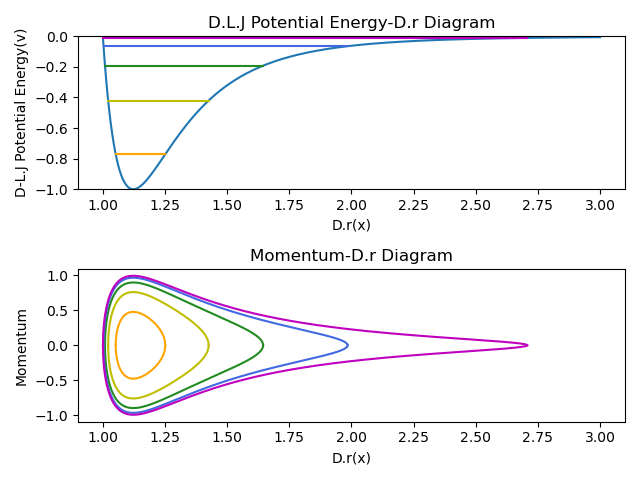
\includegraphics[scale=0.8]{h2lj.png}
            \vspace{-4mm}\caption{ $Lennard-Jones$势的能级图以及相图}
            \vspace{4mm}
            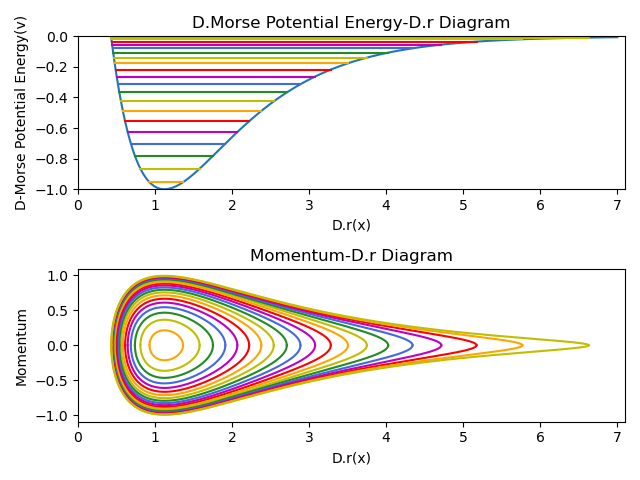
\includegraphics[scale=0.8]{h2morse.png}
            \caption{ $Morse$势的能级图以及相图}
        \end{figure} 
    }

    其中,上半部分是势能图,下半部分为$p-x$相图,可以观察到
    相图和势能图对应能级的$x_in,x_out$对应相等.


    程序实现见下(篇幅所限,程序展示只有最终结果,
    完整内容见附录)
    \begin{flushright}
        \scriptsize\emph{运行环境\\$Ubuntu 9.3.0-17\ Ubuntu1~20.04LTS$}\\
        \scriptsize\emph{$Python 3.8.8$\ \ $Anaconda 4.10.3\ \  AMD-4800u$}
            
        \end{flushright}
        \inputpython{LJ copy.py}{1}{9}
        \inputpython{LJ copy.py}{73}{78}
        \inputpython{LJ copy.py}{80}{93}
        \inputpython{Morse copy.py}{77}{86}
        \inputpython{LJ copy.py}{97}{97}
        
        \inputpython{LJ copy.py}{163}{176}



}
\subsection{结果比较}

{
    查找资料可得,氢分子振动能级势井深度为4.6eV,能级实验值如下表:


    {

    \begin{table}[h]
    \centering
    \caption{氢分子振动能级实验值}
    \begin{tabular}{@{}cccccc@{}}
    \toprule
    
    能级 & 0      & 1      & 2      & 3      & 4      \\ \midrule
    能量(eV) & -4.477 & -3.962 & -3.475 & -3.017 & -2.587 \\\cmidrule[1pt](){1-6}
    能级 & 5      & 6      & 7      & 8      & 9      \\\cmidrule(){1-6}
    能量(eV) & -2.185 & -1.811 & -1.466 & -1.151 & -0.867 \\\cmidrule[1pt](){1-6}
    能级 & 10     & 11     & 12     & 13     & 14     \\\cmidrule(){1-6}
    能量(eV) & -0.615 & -0.400 & -0.225 & -0.094 & -0.017 \\ \bottomrule
    \end{tabular}
    \end{table}
    }

    根据势井深度还原无量量纲能量进行误差处理结果如下:
    \newpage
    {
        % Please add the following required packages to your document preamble:
% \usepackage{booktabs}
% \usepackage{multirow}
\begin{table}[!h]
    \caption{$Lennard −Jones$势及$Morse$势误差表}
    \begin{tabular}{@{}c|c|c|c|c|c|c|c|c@{}}
    \toprule
    \multicolumn{4}{c|}{$Lennard −Jones$势} & {\multirow{2}{*}{能级实验值}} & \multicolumn{4}{c}{$Morse$势}       \\\cline{1-4}   \cline{6-9}
    能级  & 无量纲     & 理论值     & 误差       &                        & 误差       & 理论值    & 无量纲    & 能级 \\\hline
    0   &         &         &          & -4.477                 & 1.97\%   & -4.411 & -0.954 & 0  \\
    1   &         &         &          & -3.962                 & 0.52\%   & -4.003 & -0.866 & 1  \\
    2   & -0.772  & -3.553  & 2.25\%   & -3.475                 & 3.49\%   & -3.614 & -0.782 & 2  \\
    3   &         &         &          & -3.017                 & 6.99\%   & -3.244 & -0.702 & 3  \\
        &         &         &          &                        &          & -2.894 & -0.626 &    \\
    4   &         &         &          & -2.587                 & 1.27\%   & -2.567 & -0.555 & 4  \\
    5   &         &         &          & -2.185                 & 2.74\%   & -2.256 & -0.488 & 5  \\
    6   & -0.423  & -1.944  & 7.33\%   & -1.811                 & 8.08\%   & -1.967 & -0.426 & 6  \\
        &         &         &          &                        &          & -1.696 & -0.367 &    \\
    7   &         &         &          & -1.466                 & 1.79\%   & -1.447 & -0.313 & 7  \\
    8   &         &         &          & -1.151                 & 5.10\%   & -1.216 & -0.263 & 8  \\
        &         &         &          &                        &          & -1.005 & -0.217 &    \\
    9   & -0.196  & -0.900  & 3.76\%   & -0.867                 & 6.49\%   & -0.815 & -0.176 & 9  \\
    10  &         &         &          & -0.615                 & 4.20\%   & -0.644 & -0.139 & 10 \\
        &         &         &          &                        &          & -0.493 & -0.107 &    \\
    11  &         &         &          & -0.400                 & 9.97\%   & -0.362 & -0.078 & 11 \\
        &         &         &          &                        &          & -0.251 & -0.054 &    \\
    12  & -0.068  & -0.312  & 38.45\%  & -0.225                 & 29.46\%  & -0.160 & -0.035 & 12 \\
    13  &         &         &          & -0.094                 & 6.63\%   & -0.088 & -0.019 & 13 \\
    14  & -0.013  & -0.058  & 238.48\% & -0.017                 & 119.05\% & -0.037 & -0.008 & 14 \\ \bottomrule
    \end{tabular}
    \end{table}
    }


    \vspace{3mm}
   从\emph{表4},我们可以看出,对于氢分子,依据$ Lennard-Jones$势和
   $Morse$势作为理论基础计算出来的能级大都可以在实验数值中找到对应
   ,但是在本课题的运行环境以及程序实现中,$ Lennard-Jones$势出现
   了明显的缺级,反而$Morse$势出现了明显的多级;同时,两种位势函数
   在较高能级处均出现了较大误差,目前遇到的问题都和文献中出现或者提
   到的问题相同,并且已经相对文献减少了存在的问题与误差(
   如缺级情况
   有所改善)。目前推测问题原因可能是能级差过小同时计算
   精度不足等,具体细节会在后续讨论。
        
}

\newpage
\section{问题分析}
{
    在进行双原子分子振动能级半量子化理论的数值计算时,
    我们主要遇到了如下问题
    
    $\cdot$$\ Lennard-Jones$势的缺级

    $\cdot$$\ Morse$势的多级

    $\cdot$计算时间过长

    $\cdot$在较高能级存在较大误差

    $\cdot$求根迭代方法

    $\cdot$最优筛选问题
    
    
    下面对各个问题的进行讨论。
}
\subsection{问题产生}
{


    {\vspace{5mm}
    $\bullet${\bfseries{$Lennard-Jones$势的缺级}}
    \par $Lennard-Jones$势的缺级是比较全面的,如\emph{表4}所示
    其在不同能级均有缺级,根据引文\cite{a}\cite{b}\cite{c}
    ,可以知道在常见计算精度之下,由于$Lennard-Jones$势不够平滑,
    缺级常有发生。在计算精度不足和$Lennard-Jones$势本身缺陷下
    造成了能级的缺失。
    }


    {\vspace{5mm}
    $\bullet${\bfseries{$Morse$势的缺级}}
    \par $Lennard-Jones$势的多级,主要在高能级出现
    频繁,原因大概同样是精度的缺陷,但是仅限于猜测,具
    体原因为查阅到相关文献,准备日后进行理论分析。
    }

    {
    \vspace{5mm}
    $\bullet${\bfseries{计算时间过长}}
    \par 由于多次迭代,判断,循环,调用函数,计算量较大,
    因此计算时间过程,我们可以同过对上述内容的优化以及
    算法改进减少计算量,从而减少计算时间。
    }

    {
    \vspace{5mm}
    $\bullet${\bfseries{在较高能级存在较大误差}}
    \par 较高能级由于能级差异过小,从而容易由于收敛条件
    产上较大误差,同时由于本身数目极小,误差容易被充分展现
    ,因此应该通过迭代步长和更佳算法的选取减少误差。
    }

    {
    \vspace{5mm}
    $\bullet${\bfseries{求根迭代方法}}
    \par 由于各种求解方程的迭代法存在收敛条件,
    因而我们需要进行方程构造以及算法选取,
    $Newton$迭代法已经是一种收敛条件较弱的求根方法,
    但是仍然对构造出的函数有所限制,因为需要合理构造函数
    实现收敛求根。
    }

    {
    \vspace{5mm}
    $\bullet${\bfseries{最优筛选问题}}
    \par 对于给定的$n$,可能有不止一个
    $\varepsilon_n$满足精度要求,在循环中我们需要考虑
    如何筛选出最优解并进行储存与输出。
    }

    
}
\subsection{解决方案}
{


    {\vspace{5mm}
    $\bullet${\bfseries{$Lennard-Jones$势的缺级}}
    \par 由于问题产生原因是势函数的缺陷以及精度不足,因此我们
    在计算中应该提升精度,或者改变为更准确优秀的位势函数
    ,如本题中用$Morse$势代替$Lennard-Jones$势
    便可解决缺级问题。
    }


    {\vspace{5mm}
    $\bullet${\bfseries{$Morse$势的缺级}}
    \par 同样的,多级问题也可以通过改变计算精度,
    取更好的$a$值,以及改进位势函数得到,查阅文献
    \cite{a},了解到$Varshni$或许可以更好的描述
    本题目描述运动情况的势能,如有需要可以尝试
    用此修正。
    }

    {
    \vspace{5mm}
    $\bullet${\bfseries{计算时间过长}}
    \par 减少迭代循环次数,优化算法等都可以加快计算
    减少循环次数可以通过构造合理函数,合理优化算法减少
    $\varepsilon_n$增加次数(不重复计算不可能的数值)
    等方法,优化算法可以通过改进计算方法,调用更好的函数表达形式,
    用更稳定的数学包(例如用$numpy.math$而不是$math$)
    ,画图取合适的上下限等等。
    }

    {
    \vspace{5mm}
    $\bullet${\bfseries{在较高能级存在较大误差}}
    \par 较高能级由于能级差异过小,因此我们需要大量提升精度,
    常规的均匀梯度精度明显不足,因此需要动态梯度在$\varepsilon_0\to 0$
    时减少步长以此增加精度。
    }

    {
    \vspace{5mm}
    $\bullet${\bfseries{求根迭代方法}}
    \par 选用收敛条件较弱的牛顿迭代法,构造合适的
    迭代函数,(用低幂次的迭代函数为好)可以极大的提升收敛速度,
    如有需要,可以采用$Aitken$加速法再行加速。
    }

    {
    \vspace{5mm}
    $\bullet${\bfseries{最优筛选问题}}
    \par 对于多个$\varepsilon_n$满足精度的情况,
    可以用一个列表进行收纳,本次循环结束之后,再行
    寻找最优数值并输出到结果列表,便可得到对于每个$n$,最合适的
    $\varepsilon_n$值。
    }

    
}



\newpage

\begin{thebibliography}{99}
    \bibitem{a}熊志斌. \emph{$H_2$分子振动能级的数值模拟.pdf}[M]. 湖南师范大学 数学与计算机科学学院,湖南 长沙,湖 南 文 理 学 院 学 报(自 然 科 学 版) 第 17卷 第三期 2005年9月
    \bibitem{b}张磬兰;王燕昌 . \emph{双原子分子振动能级半量子化及量子理论的数值计算}[M]. 宁夏大学物理系;宁夏大学物理系 \ 来源:大学物理 ISSN:1000-0712 年:1997 卷:016 期:001
    \bibitem{c}彭芳麟. \emph{计算物理基础}[M]. 高等教育出版社
    
\end{thebibliography}

\newpage

\begin{appendices}


    \renewcommand{\thesection}{\Alph{section}}
    \section{全部程序实现}


\subsection{\emph{Lennard-Jones}势理论程序实现}
{
    \begin{flushright}
        \scriptsize\emph{运行环境\\$Ubuntu 9.3.0-17\ Ubuntu1~20.04LTS$}\\
        \scriptsize\emph{$Python 3.8.8$\ \ $Anaconda 4.10.3\ \  AMD-4800u$}
            
        \end{flushright}
        \inputpython{LJ copy.py}{1}{176}

}
\subsection{\emph{Morse}势理论程序实现}
{
    \begin{flushright}
        \scriptsize\emph{运行环境\\$Ubuntu 9.3.0-17\ Ubuntu1~20.04LTS$}\\
        \scriptsize\emph{$Python 3.8.8$\ \ $Anaconda 4.10.3\ \  AMD-4800u$}
            
        \end{flushright}
        \inputpython{Morse copy.py}{1}{176}

}
    
\newpage
\renewcommand{\thesection}{\Alph{section}}
    \section{图片结果输出}

    \subsection{$H_2$分子振动能级}
    \subsubsection{\emph{Lennard-Jones}势}
    {
        \begin{figure}[!ht]
            \caption{ $Lennard-Jones$势能级图}
            \centering
            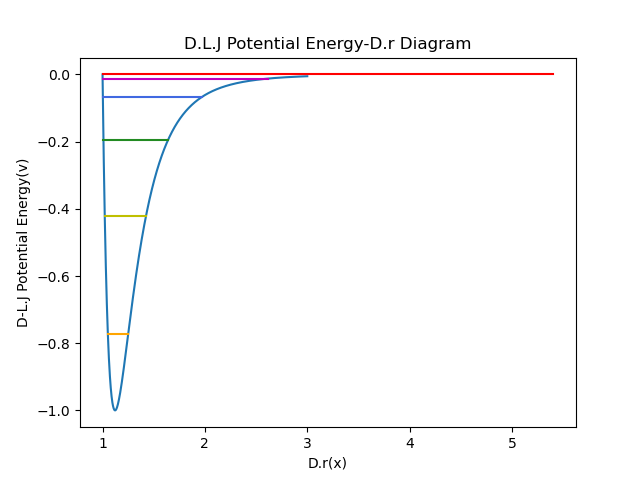
\includegraphics[scale=0.75]{h21.png}
        \end{figure} 
        \begin{figure}[!ht]
            \caption{ $Lennard-Jones$势相图}
	
            \centering
            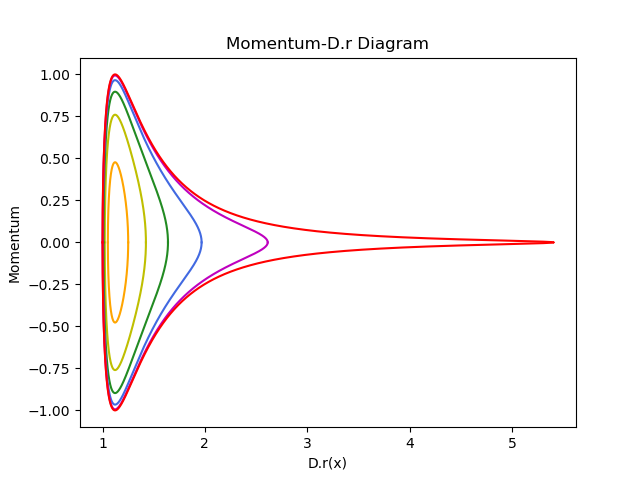
\includegraphics[scale=0.75]{h22.png}
        \end{figure} 
        \begin{figure}[!ht]
            \caption{ $Lennard-Jones$势能级图及相图}
	
            \centering
            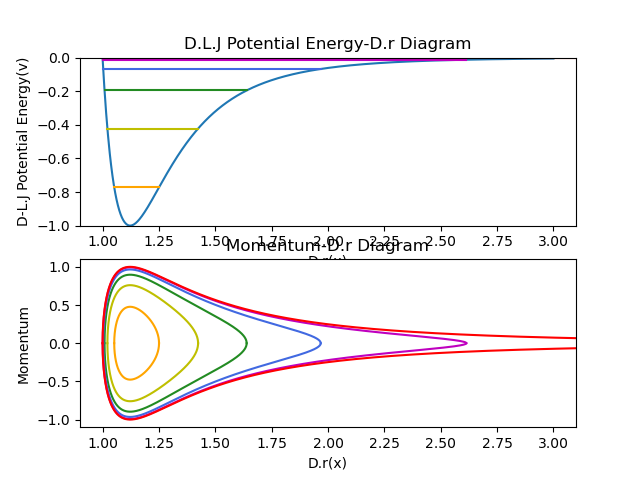
\includegraphics[scale=0.75]{h23.png}
        \end{figure} 
    }
    \subsubsection{\emph{Morse}势}
    {
        \begin{figure}[!ht]
            \caption{ $Morse$势能级图}
            \centering
            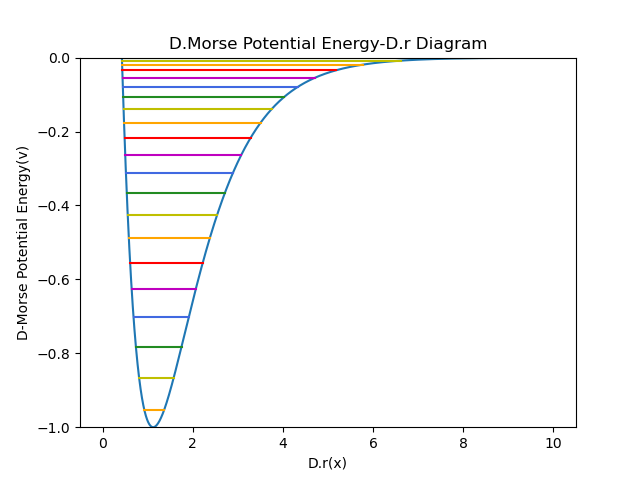
\includegraphics[scale=0.75]{h2-1.png}
        \end{figure} 
        \begin{figure}[!ht]
            \caption{ $Morse$势相图}
	
            \centering
            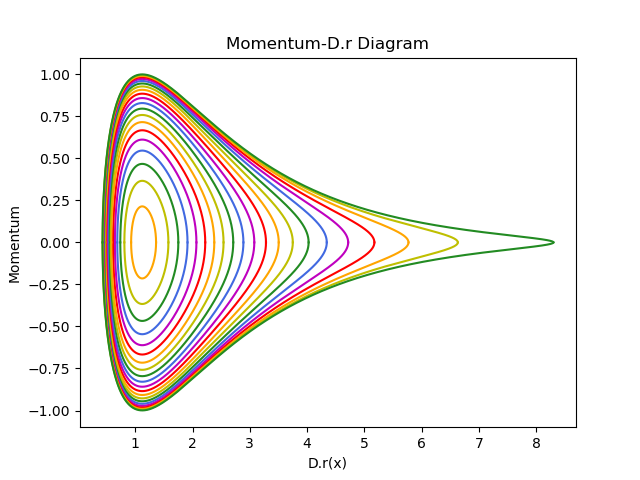
\includegraphics[scale=0.75]{h2-2.png}
        \end{figure} 
        \begin{figure}[!ht]
            \caption{ $Morse$势能级图及相图}
	
            \centering
            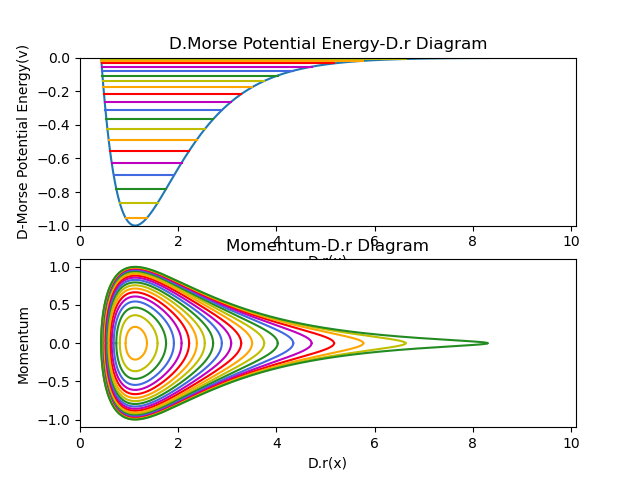
\includegraphics[scale=0.75]{h2-3.png}
        \end{figure} 
    }

        \newpage
    \subsection{$DH$分子振动能级}
    \subsubsection{\emph{Lennard-Jones}势}
    {\newpage
        \begin{figure}[!ht]
            \caption{ $Lennard-Jones$势能级图}
            \centering
            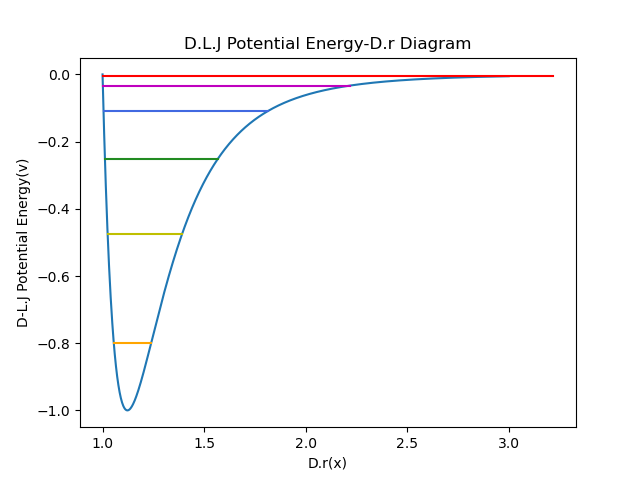
\includegraphics[scale=0.75]{dh1.png}
        \end{figure} 
        \begin{figure}[!ht]
            \caption{ $Lennard-Jones$势相图}
	
            \centering
            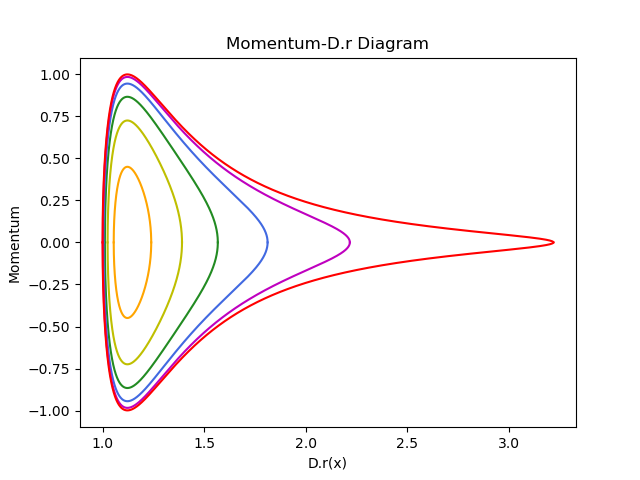
\includegraphics[scale=0.75]{dh2.png}
        \end{figure} 
        \begin{figure}[!ht]
            \caption{ $Lennard-Jones$势能级图及相图}
	
            \centering
            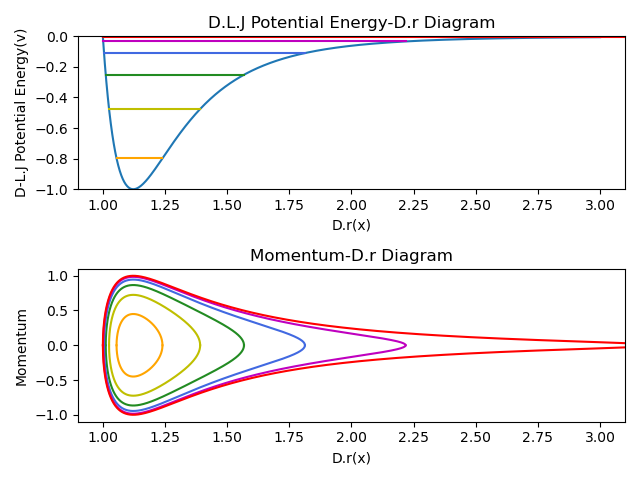
\includegraphics[scale=0.75]{dh3.png}
        \end{figure} 
    }
    \newpage\subsubsection{\emph{Morse}势}
    {
        \begin{figure}[!ht]
            \caption{ $Morse$势能级图}
            \centering
            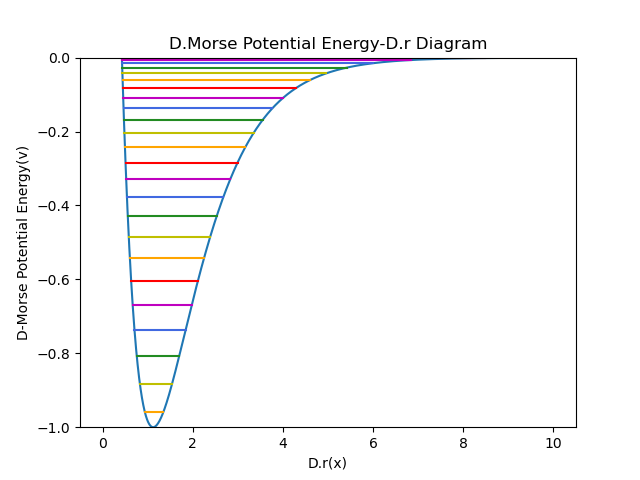
\includegraphics[scale=0.75]{dh-1.png}
        \end{figure} 
        \begin{figure}[!ht]
            \caption{ $Morse$势相图}
	
            \centering
            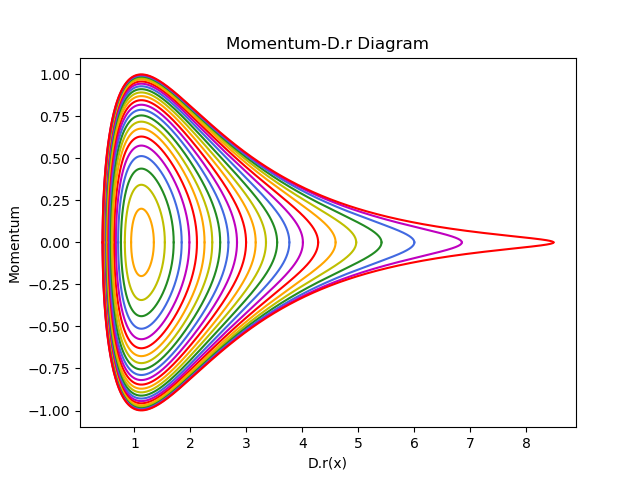
\includegraphics[scale=0.75]{dh-2.png}
        \end{figure} 
        \begin{figure}[!ht]
            \caption{ $Morse$势能级图及相图}
	
            \centering
            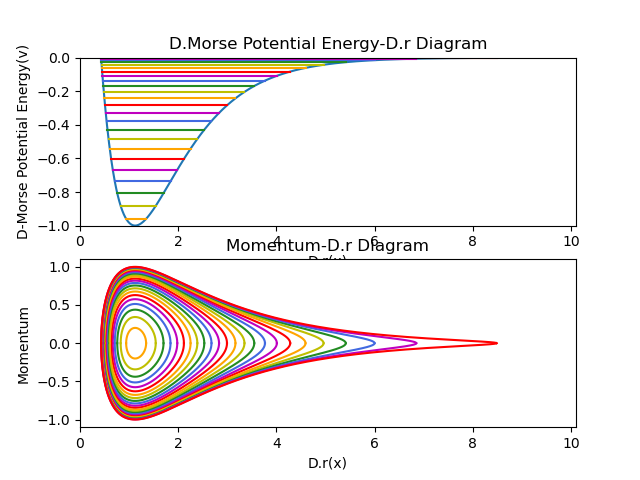
\includegraphics[scale=0.75]{dh-3.png}
        \end{figure} 
    }
    \newpage
    \subsection{$O_2$分子振动能级}
    {
        \subsubsection{\emph{Lennard-Jones}势}
        {\newpage
            \begin{figure}[!ht]
                \caption{ $Lennard-Jones$势能级图}
                \centering
                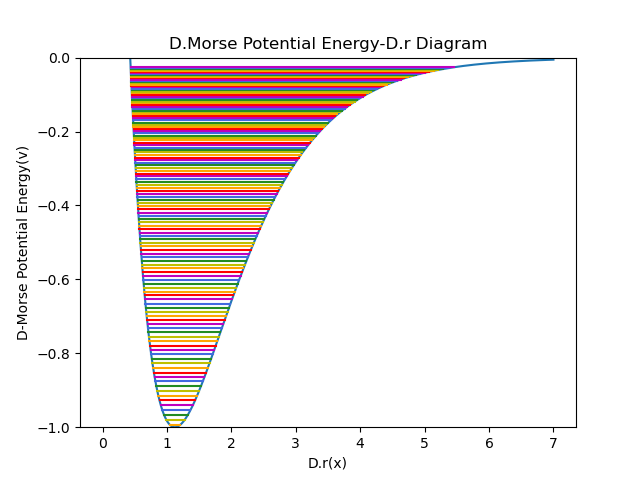
\includegraphics[scale=0.75]{021.png}
            \end{figure} 
            \begin{figure}[!ht]
                \caption{ $Lennard-Jones$势相图}
        
                \centering
                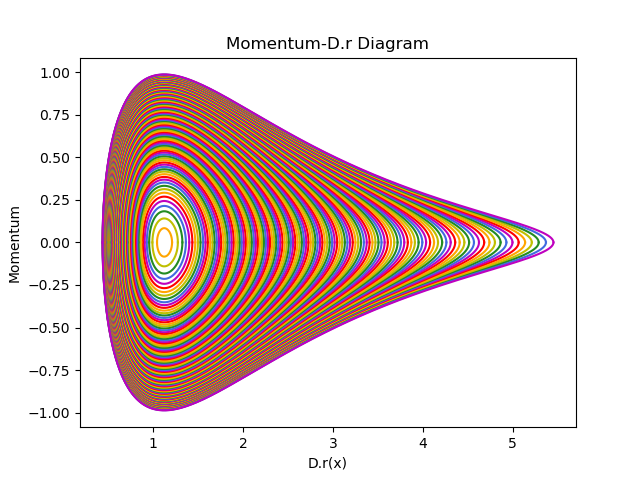
\includegraphics[scale=0.75]{022.png}
            \end{figure} 
            \begin{figure}[!ht]
                \caption{ $Lennard-Jones$势能级图及相图}
        
                \centering
                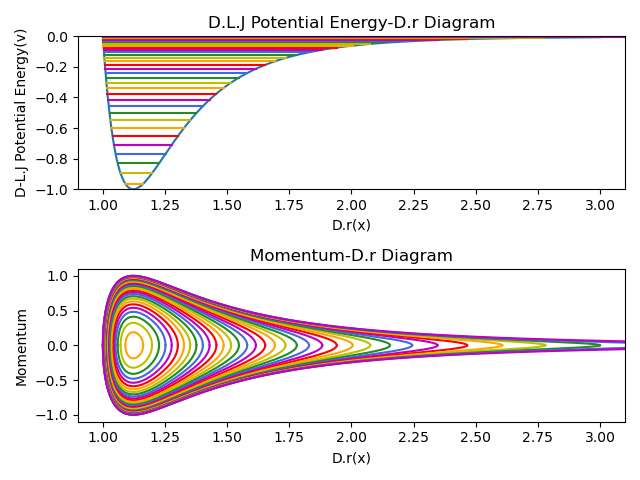
\includegraphics[scale=0.75]{023.png}
            \end{figure} 
        }
        \newpage\subsubsection{\emph{Morse}势}
        {
            \begin{figure}[!ht]
                \caption{ $Morse$势能级图}
                \centering
                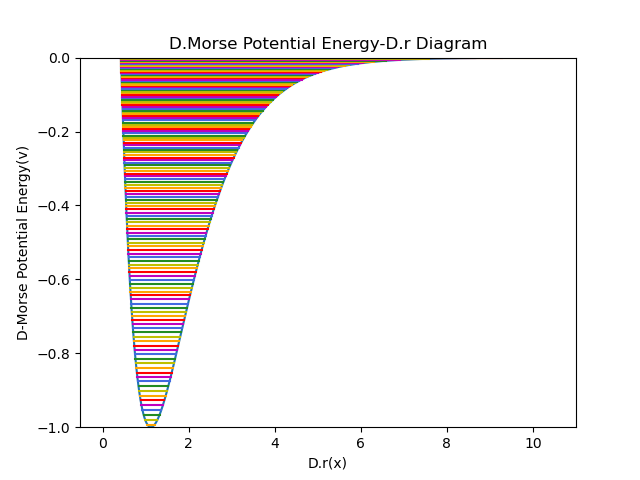
\includegraphics[scale=0.75]{02-1.png}
            \end{figure} 
            \begin{figure}[!ht]
                \caption{ $Morse$势相图}
        
                \centering
                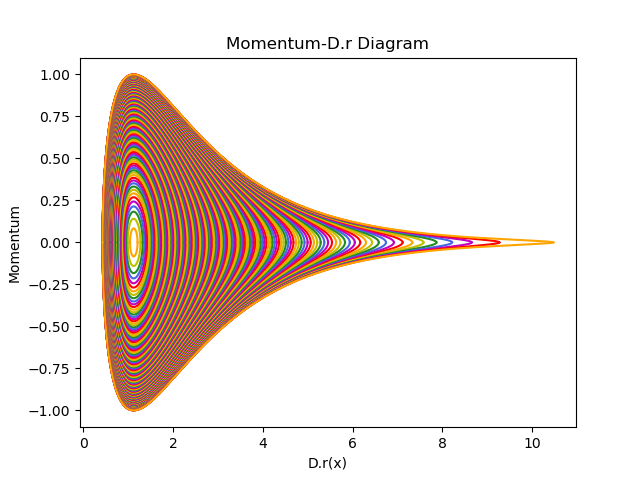
\includegraphics[scale=0.75]{02-2.png}
            \end{figure} 
            \begin{figure}[!ht]
                \caption{ $Morse$势能级图及相图}
        
                \centering
                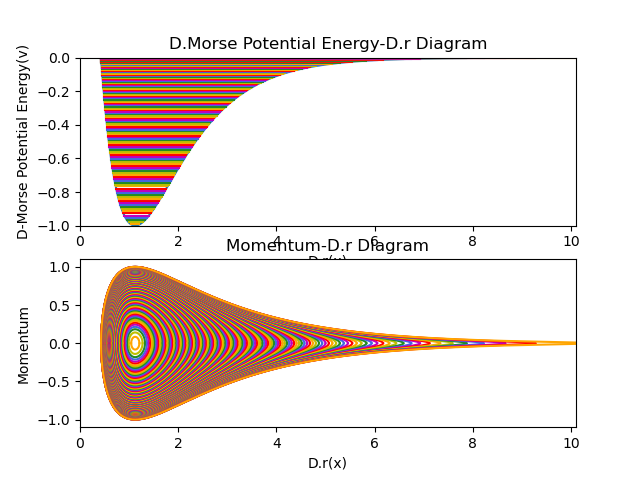
\includegraphics[scale=0.75]{02-3.png}
            \end{figure} 
        }
    }

\end{appendices}

\end{document}